\chapter{Introduzione}
Il mondo sta diventando sempre più interconnesso. Troviamo dispositivi connessi in quasi tutte le case e le reti informatiche sono il sistema nervoso delle organizzazioni aziendali e governative di tutto il mondo. Purtroppo per gli investigatori, Internet è stata progettata per la robustezza e la ridondanza, piuttosto che per la sicurezza e la tracciabilità. Questo aumenta la complessità e l'incertezza delle indagini digitali e rappresenta un'ardua sfida per gli informatici forensi. La digital forensics sta diventando sempre più importante con l'aumento del cybercrimine e di altri gravi reati informatici. Le prove digitali sono ovunque e svolgono un ruolo importante in quasi tutte le indagini penali come: piccoli reati, cybercrimine, crimine organizzato e anche il terrorismo. È quindi fondamentale che gli studenti di informatica e sicurezza acquisiscano una buona conoscenza della digital forensics, per poter agire come esperti in un contesto legale.

\section{Forensic Science}
\begin{figure}[h]
    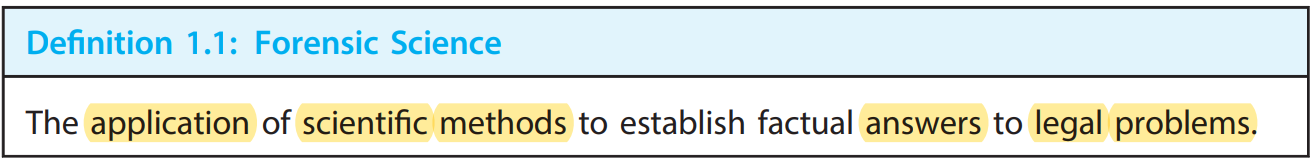
\includegraphics[width=\textwidth]{Capitolo 1/Figure/forensic-science-def.png}
\end{figure}

Le Forensic Science sono \textbf{l'applicazione di metodi scientifici che permettono di rispondere a problemi legali.}
Uno scienziato forense deve stabilire il cosa, il come, il chi e il quando; e per offrire queste risposte utilizza tool e strumenti relativi a scienze teoriche e applicate. Tuttavia non è sempre possibile ottenere la certezza totale per queste risposte e quindi uno scienziato forense a volte deve far ricorso a metodi statistici e probabilistici.

\subsection{Principio di scambio di Locard}
Edmond Locard ha formulato il famoso \textbf{Locard’s Exchange Principle}, che è alla base degli studi delle scienze forensi. Il principio afferma che 
\begin{quote}
    \textit{"quando persone o oggetti entrano in contatto tra loro avviene un passaggio incrociato di materiale."}
\end{quote}

\begin{figure}[h]
    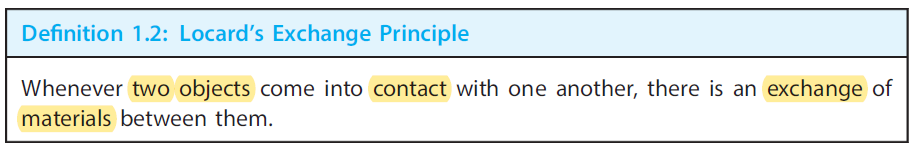
\includegraphics[width=\textwidth]{Capitolo 1/Figure/locard-principle.png}
\end{figure}
Questo scambio di materiale è essenziale perché genera tracce e prove utili per la ricostruzione e l'identificazione di un crimine.

\subsection{Ricostruzione del crimine}
La ricostruzione della scena del crimine è il processo che determina le ipotesi e la sequenza degli eventi  attraverso metodi scientifici. 
\begin{figure}[h]
    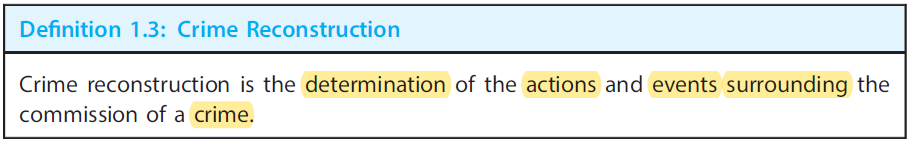
\includegraphics[width=\textwidth]{Capitolo 1/Figure/crime-recostruction-def.png}
\end{figure}

L'obiettivo della ricostruzione di un crimine è stabilire delle ipotesi e successivamente testarne la veridicità. Se un'ipotesi viene confermata allora può essere fornita una possibile spiegazione al crimine; altrimenti, se viene rifiutata, si passa a considerare le altre possibili ipotesi.

\clearpage
\subsection{Investigazione}
Il processo di investigazione è un'analisi sistematica con l'obiettivo di identificare i fatti chiave di un crimine attraverso comuni metodologie come le 5WH.
\begin{figure}[h!]
    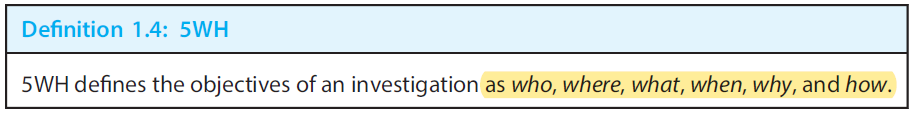
\includegraphics[width=\textwidth]{Capitolo 1/Figure/5WH-def.png}
\end{figure}

\begin{itemize}
    \item Who: persone coinvolte, compresi sospettati, complici e vittime.
    \item Where: Le location rilevanti.
    \item What: Descrizione dei fatti accaduti.
    \item When: timeline degli eventi.
    \item Why: Le motivazioni e perché è successo in un dato momento.
    \item How: Come è stato commesso.
\end{itemize}

\subsection{Evidence Dynamics}
\begin{figure}[h!]
    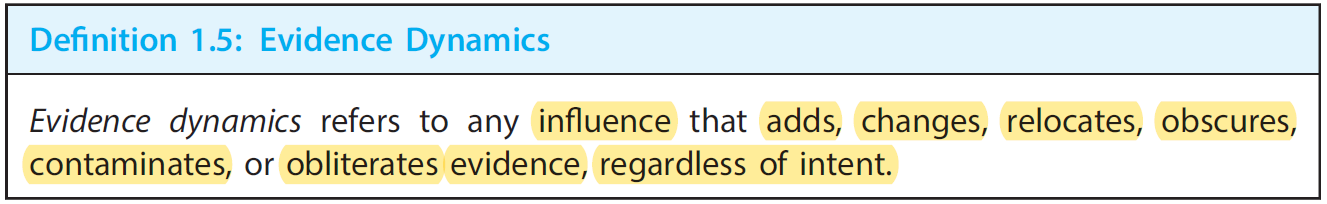
\includegraphics[width=\textwidth]{Capitolo 1/Figure/evidence-dynamic.png}
\end{figure}
In rari casi un investigatore o uno scienziato forense avranno l'opportunità di esaminare la scena del crimine nel suo stato originale, piuttosto andranno in contro a una dinamica delle prove.
Le dinamiche delle prove consistono in qualsiasi azione, intenzionale o non, atta ad aggiungere, cambiare, oscurare, contaminare, eliminare le prove.
Nel campo della digital forensic una dinamica potrebbe essere la cancellazione di un dato settore dell' HDD.

\clearpage
\section{Digital Forensics}
\begin{figure}[h!]
    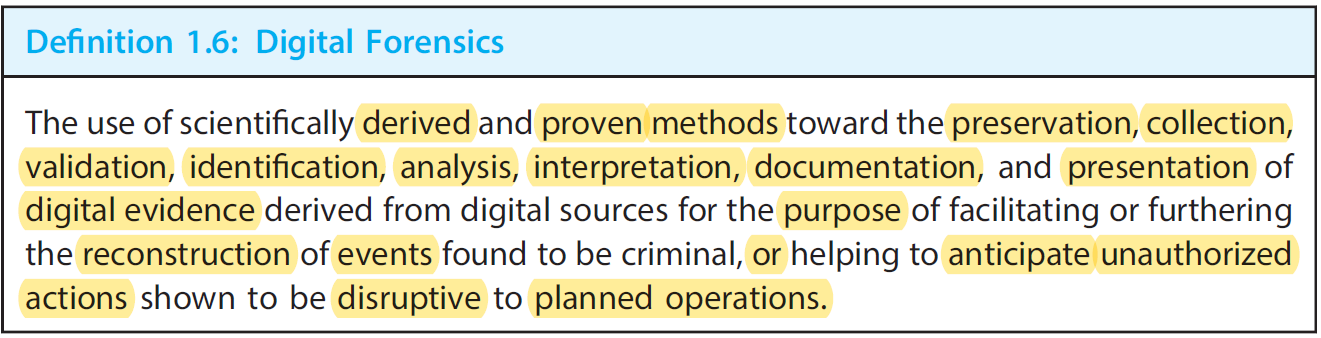
\includegraphics[width=\textwidth]{Capitolo 1/Figure/digital-forensics-def.png}
\end{figure}
L'obiettivo solitamente è raccogliere dati(prove) per comprendere il comportamento umano, ma per interpretare le prove digitali il prerequisito è comprendere come i sistemi informatici si comportano e perché. 
È importante notare che le prove digitali possono essere volatili e facilmente manipolabili, quindi nella digital forensics è essenziale una conservazione affidabile delle prove.
Inoltre dovendo rispondere a problemi legali è necessario garantire solidità e robustezza all'investigazione e la sua conclusione.
La keyword per la raccolta, interpretazione e presentazioni delle prove in tribunale è l'\textbf{ammissibilità delle prove.}

\subsection{Crimini e incidenti(sinistri)}
La Digital Forensics è applicata sia in un contesto di diritto penale sia diritto civile. Per il diritto penale si parla di \textbf{crimini}; per il diritto civile si parla di \textbf{incidenti o sinistri.}

\subsection{Digital Devices, Media, and Objects}
I Digital Devices sono dispositivi fisici come un laptop, uno smartphone o una macchina. Questi contengono una memoria di archiviazione che prende il nome di Digital Media. I Digital Media contengono dati in formato binario che prendono il nome di Digital Data. Un insieme strutturato di Digital Data prende nome di Digital Object.
\begin{figure}[h!]
    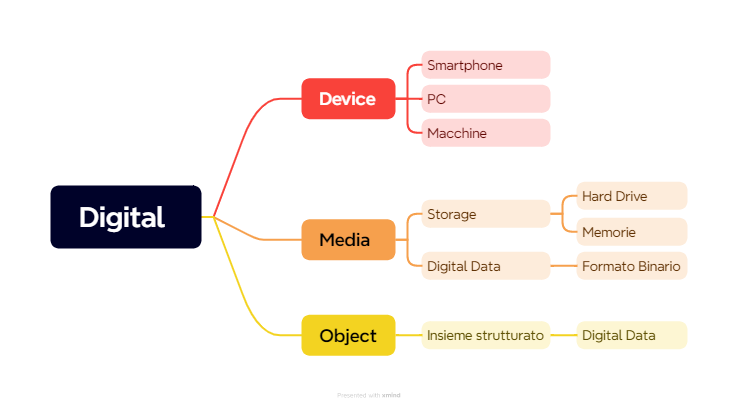
\includegraphics[width=\textwidth]{Capitolo 1/Figure/schema-digital-devices-media-object.png}
\end{figure}

\clearpage
\subsection{Validità forense e principi fondamentali}
\begin{figure}[h!]
    \includegraphics[width=\textwidth]{Capitolo 1/Figure/forensic-solidità.png}
\end{figure}

Un'indagine forense risulta valida se rispetta gli standard e principi consolidati.
I due principi fondamentali di un'indagine forense sono: \textit{\textbf{l'integrità delle prove (evidence integrity)} e \textbf{la catena di custodia (chain of custody).}}

L'integrità delle prove si riferisce alla conservazione delle prove nella loro forma originale.
Dato che garantire quest'integrità non è sempre possibile, è importante documentare scrupolosamente tutti gli step dell'investigazione, attraverso una catena di custodia.
La catena di custodia si riferisce alla documentazione rigorosa dell'acquisizione, controllo, analisi e disposizione delle prove.

\begin{figure}[h!]
    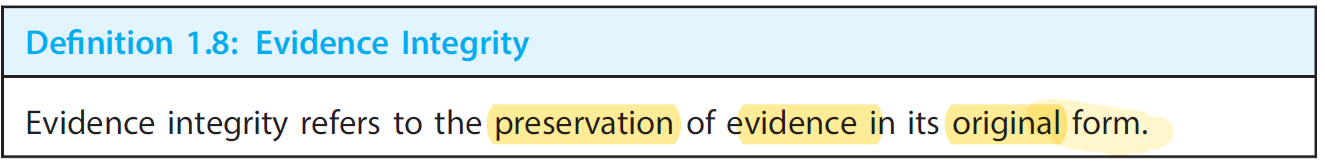
\includegraphics[width=\textwidth]{Capitolo 1/Figure/evidence-integrity.png}
\end{figure}

\begin{figure}[h!]
    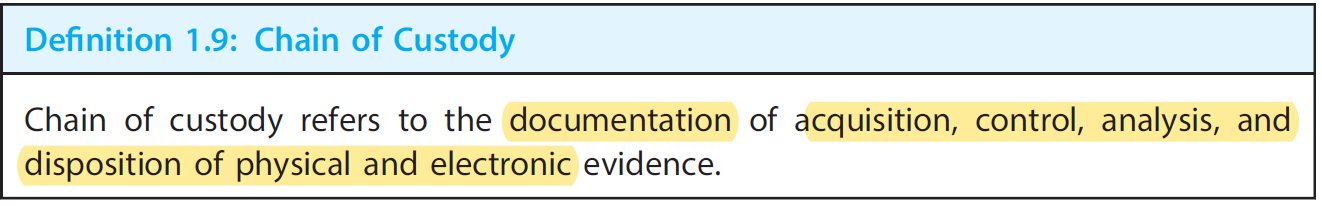
\includegraphics[width=\textwidth]{Capitolo 1/Figure/chain-of-custody.png}
\end{figure}

\paragraph{Nota bene}
Sarebbe utile evitare troppi passaggi di custodia e limitare l'accesso alle prove soprattutto da soggetti non autorizzati.

\subsection{Ricostruzione del crimine nella Digital Forensics}
Nella Digital Forensics la ricostruzione di un crimine si divide solitamente in 5 step:
\begin{itemize}
    \item Analisi delle prove
    \item Classificare il ruolo di una prova come causa effetto di un evento
    \item Costruire gli eventi e testare la validità
    \item Combinare gli eventi per creare una catena
    \item Testare le ipotesi con metodi scientifici
\end{itemize}


\section{Prove Digitali}
\begin{figure}[h!]
    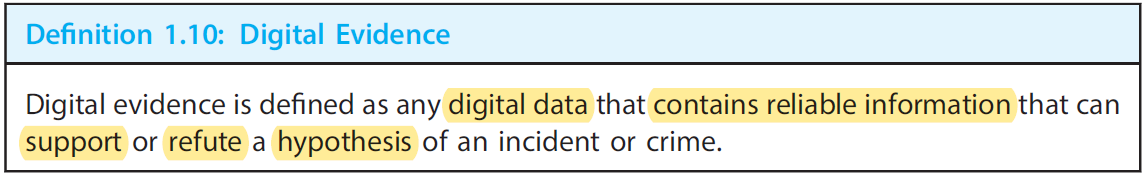
\includegraphics[width=\textwidth]{Capitolo 1/Figure/digital-evidence.png}
\end{figure}
È importante conservare le prove digitali in modo da preservarne l'integrità e l'ammissibilità in tribunale.

\subsection{Metadata}
I Metadata contengono informazioni riguardo i Data Object. Ad esempio i Metadata associato ad una fotografia può contenere informazioni sul modello di macchina fotografica, sulla data, il luogo e su chi ha scattato la foto.
Analizzare con attenzione i Metadata può portare alla scoperta di informazioni chiave utili nella risoluzione di un processo di investigazione forense.